\documentclass[12pt]{article}

\usepackage{sbc-template}

\usepackage{graphicx,url}
\usepackage[brazil]{babel}   
%\usepackage[latin1]{inputenc}  
\usepackage[utf8]{inputenc}
\usepackage{import}
% UTF-8 encoding is recommended by ShareLaTex

     
\sloppy

\title{A survey into CDNs Security}

\author{Lucas Begnini Costa\inst{1}, Carlos A. Maziero\inst{1}}


\address{LARSIS - Departamento de Informatica -- Universidade Federal do Paran\'a
  (UFPR)\\
 Curitiba -- PR -- Brazil
 \email{lucasbegnini@gmail.com,}
}

\begin{document} 

\maketitle

\begin{abstract}
  This meta-paper describes the style to be used in articles and short papers
  for SBC conferences. For papers in English, you should add just an abstract
  while for the papers in Portuguese, we also ask for an abstract in
  Portuguese (``resumo''). In both cases, abstracts should not have more than
  10 lines and must be in the first page of the paper.
\end{abstract}
     
\begin{resumo} 
  Este meta-artigo descreve o estilo a ser usado na confecção de artigos e
  resumos de artigos para publicação nos anais das conferências organizadas
  pela SBC. É solicitada a escrita de resumo e abstract apenas para os artigos
  escritos em português. Artigos em inglês deverão apresentar apenas abstract.
  Nos dois casos, o autor deve tomar cuidado para que o resumo (e o abstract)
  não ultrapassem 10 linhas cada, sendo que ambos devem estar na primeira
  página do artigo.
\end{resumo}


\section{Introdu\c{c}\~ao}


Vivemos em um mundo rodeado de tecnologia, onde a cada dia somos surpreendidos com uma coisa totalmente inovadora, disruptiva. Uma era onde a internet foi respons\'avel por atravessar mares, superar dist\^ancias e at\'e mesmo idiomas. Hoje se pode comunicar em tempo real com pessoas que est\~ao em lados completamente opostos ao seu. 
\newline
Hoje \'e poss\'ivel que empresas estrangeiras muito distantes fisicamente, como China, India, EUA e etc, forne\c{c}am servi\c{c}os para regi\~oes mais remotas do mundo. Isso inclui servi{c}os de multim\'idia como armazenamento de fotos, de v\'ideos e at\'e conte\'udos de consumo instant\^aneo.
\newline
Esse encurtamento de dist\^ancia pode parecer simples, mas vem de um sistema complexo que visa fornecer ao usu\'ario final uma experi\^encia agrad\'avel com conte\'udos entregues de maneira satifat\'oria mas sem, necessariamente, replica-lo por todo o globo. O que nos leva a dizer que uma CDN(\textit{Content Delivery Network} ) \'e uma rede de distribui\c{c}\~ao de conte\'udo que tem como objetivo fornecer ao usu\'ario de aplica\c{c}\~oes globais uma experi\^encia satisfat\'oria na utiliza\c{c}\~ao de servi\c{c}os, principalmente sob demanda.
\begin{figure}[H]
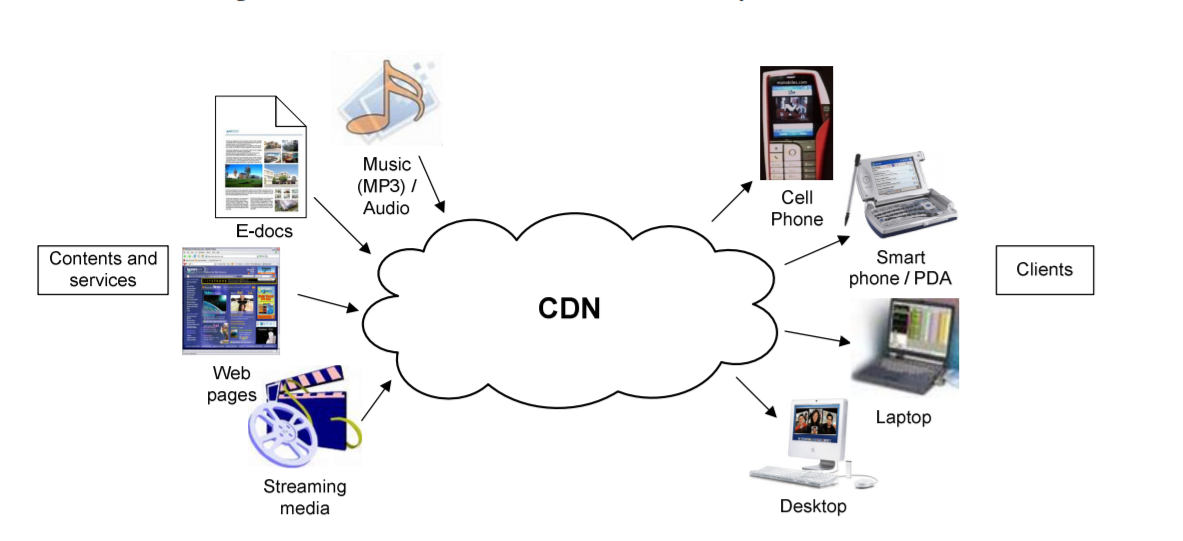
\includegraphics[height=7cm]{Figuras/contextualizacao.png} 
\label{figura:contextualizacao} 
\end{figure}
Temos v\'arios servi\c{c}os que se utiliza no dia a dia onde essa no\c{c}\~ao de CDN \'e completamente abstrata ao usu\'ario final. Como servi\c{c}os de Video-On-Demand de empresas de TV, spotify, Amazon Prime Video e at\'e Netflix, como \'e mostrado no artigo do \cite{adhikari2012unreeling}.
\newline
Existem hoje diversas empresas que fornecem esse servi\c{c}o ao redor do globo. Como:
\begin{itemize}
\item Akamai;
\item Limelight;
\item Level 3;
\item e etc.
\end{itemize}

Essas tr\^es redes s\~ao hoje, as principais fornecedoras de servi\c{c}o de CDN da Netflix. Cada um com um caracter\'istica e voltado pra um p\'ublico.
\subsection{AKAMAI}
\paragraph{Origem}- Massachusetts Institute of Technology (MIT), em 1995, com Tim Berners-Lee.
\paragraph{Pontos de atua\c{c}\~ao}
\begin{figure}[H]
\caption{Rede de distribui\c{c}\~ao Akamai}
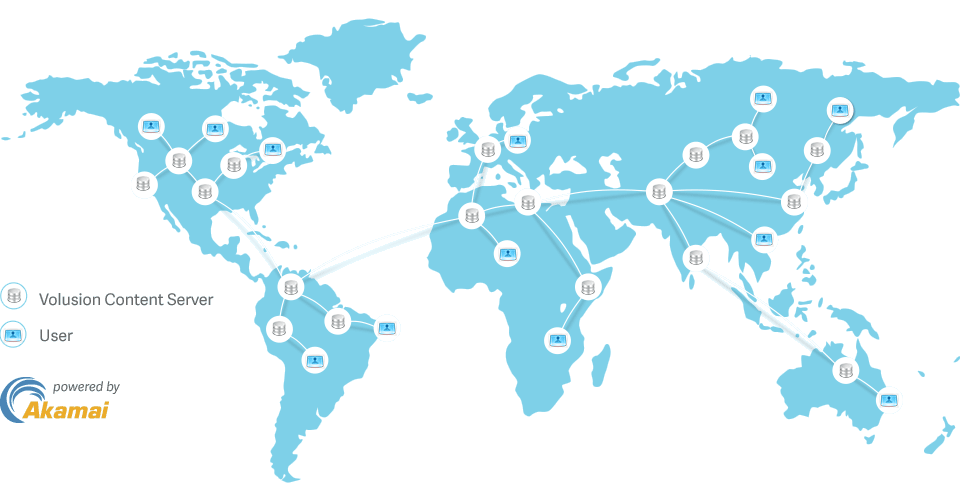
\includegraphics[width=12cm]{Figuras/akamai_map.png} 
\label{figura:akamai_map}
\end{figure}
\paragraph{Principais clientes}- Adobe, Airbnb, American Idol, Audi, Autodesk, EMC2, e muitas outras.
\subsection{Limelight}
\paragraph{Origem}- Tempe, Arizona, EUA.
\paragraph{Pontos de atua\c{c}\~ao}
\begin{figure}[H]
\caption{Rede de distribui\c{c}\~ao Limelight}
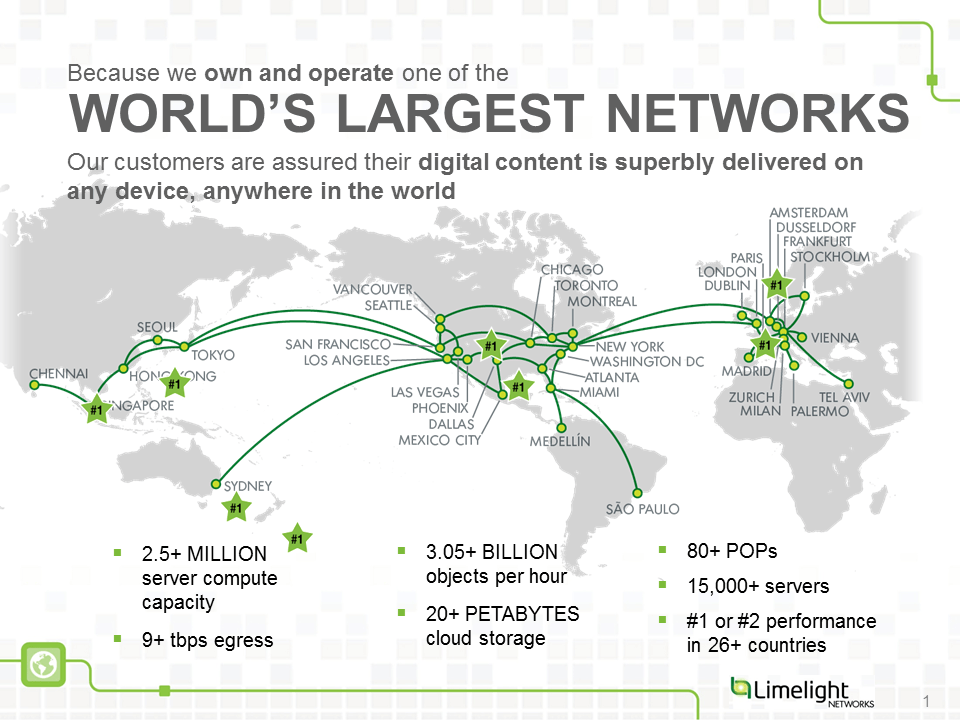
\includegraphics[width=12cm]{Figuras/limelight_map.png} 
\label{figura:limelight_map}
\end{figure}
\paragraph{Principais clientes}- N\~ao informado.
\subsection{Level 3}
\paragraph{Origem}- Monroe, Luisiana, EUA. 
\paragraph{Pontos de atua\c{c}\~ao}
\begin{figure}[H]
\caption{Rede de distribui\c{c}\~ao Level 3}
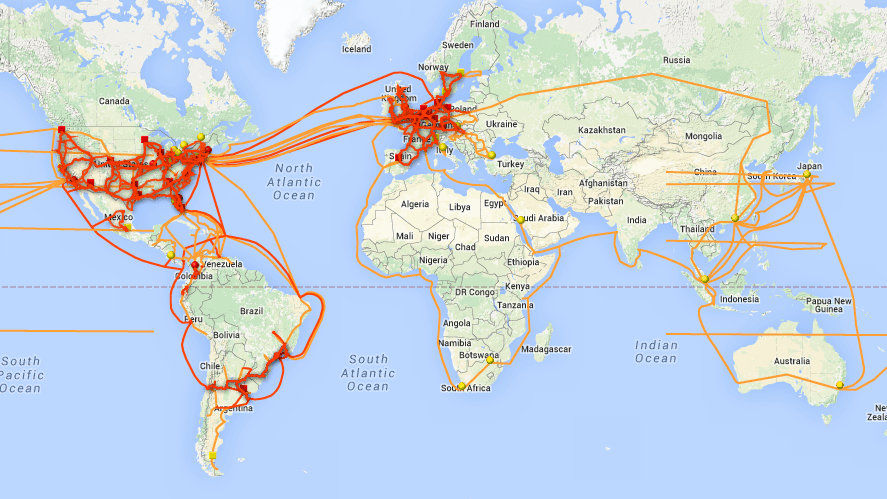
\includegraphics[width=12cm]{Figuras/level3_map.png} 
\label{figura:level3_map}
\end{figure}
\paragraph{Principais clientes}- N\~ao informado.
\subsection{Vis\~ao geral}
Todas essas redes se concentram praticamente no mesmo ponto. \'E claro, movida por uma quest\~ao financeira, todas elas est\~ao basicamente concentradas nos Estados Unidos, Europa e algumas adentram at\'e o mercado asi\'atico.
\newline
Nesse artigo vamos tentar entender um pouco mais a respeito de CDNs e tamb\'em um pouco do seu sistema de seguran\c{c}a. Sendo assim, poderemos dividir o restante desse artigo em duas partes: A primeira ser\'a relacionada somente a composi\c{c}\~ao da CDN, ou seja, tudo aquilo que \'e necess\'ario para se constituir uma CDN. Na segunda etapa falaremos primeiro um pouco sobre seguran\c{c}a em um \^ambito geral e depois aprofundaremos em seus conceitos voltados para CDN.

\section{Composi\c{c}\~ao de uma CDN} \label{sec:composicao}
Para entendermos melhor uma CDN precisamos primeiro estricha-la em v\'arios pequenos peda\c{c}os para assim compreende-la em uma maneira totalit\'aria.
\newline
Uma CDN apesar de abstratamente ser vista como um mecanismo \'unico ela pode ser vista como a soma de v\'arios tipos de elementos, v\'arias caracter\'isticas que somadas e configuradas formar\'a um mecanismo \'unico e transparente ao usu\'arios. Caracter\'isticas essas que s\~ao:
\begin{itemize}
\item Organiza\c{c}\~ao;
\item Servidores;
\item Protocolos de iter\c{c}\~oes;
\item E tipos de conte\'udo.
\end{itemize}

\paragraph{Organiza\c{c}\~ao}- Quanto a organiza\c{c}\~ao uma CDN pode ser uma rede puramente CDN ou uma rede \textit{overlay}, que nada mais \'e que uma rede onde ela tenta abstrai as camadas de redes j\'a existentes(como transporte, redes e etc) e transforma-l\'a em uma rede puramente CDN.

\paragraph{Tipos de conte\'udos}- O tipos de conte\'udo que ir\~ao ser transportados dentro da rede s\~ao fundamentais para definir diversos aspectos de configura\c{c}\~oes que ser\~ao utilizadas dentro da rede. Como por exemplo, a forma de Cache que ser\'a feita os arquivos ou at\'e mesmo a forma como v\~ao ser distribu\'idos esses mesmos conte\'udos, se ser\~ao distribu\'idos em conjunto ou em partes como o caso de uma pagina HTML que possui um video para cada regi\~ao do  mundo. Todos os outros pontos levam em conta primeiro o tipo de conte\'udo para definir quais ser\~ao suas escolhas.
\newline
Os demais itens ser\~ao tratados nos pr\'oximos pontos. Tipos de servidores em \ref{section:tipos_de_servidores} e protocolos de itera\c{c}\~oes em \ref{section:protocolos_interacoes}

\subimport{composicao/}{tiposServidores}

\subimport{composicao/}{protocolosInteracoes}

\subimport{composicao/}{selecaoEntrega}


\section{Seguran\c{c}a de uma CDN} \label{sec:seguranca}
Segundo \cite{ferreira2004novo} seguran\c{c}a \'e definido como um conjunto de a\c{c}\~oes que e dos recursos utilizados para proteger algo ou algu\'em, ou, o que serve para diminuir os riscos ou perigo. Portanto, seguran\c{c}a \'e um tema extramente abrangente e complexo. Podemos falar de t\'opicos como seguran\c{c}a f\'isica, social, de um sistema ou at\'e mesmo de um grupo de servidores interconectados, que \'e o caso da CDN, e ainda coloca-los todos dentro do mesmo grupo. Ou seja, podemos trat\'a-los de forma separada ou analisando o conjunto todo.
\paragraph{} 
Ainda dentro de Seguran\c{c}a de CDN podemos tratar de pontos principais, onde o vazamento \'e ponto crucial e mais l\'ogico de ser atacado. 
\begin{figure}[H]
\caption{Seguran\c{c}a}
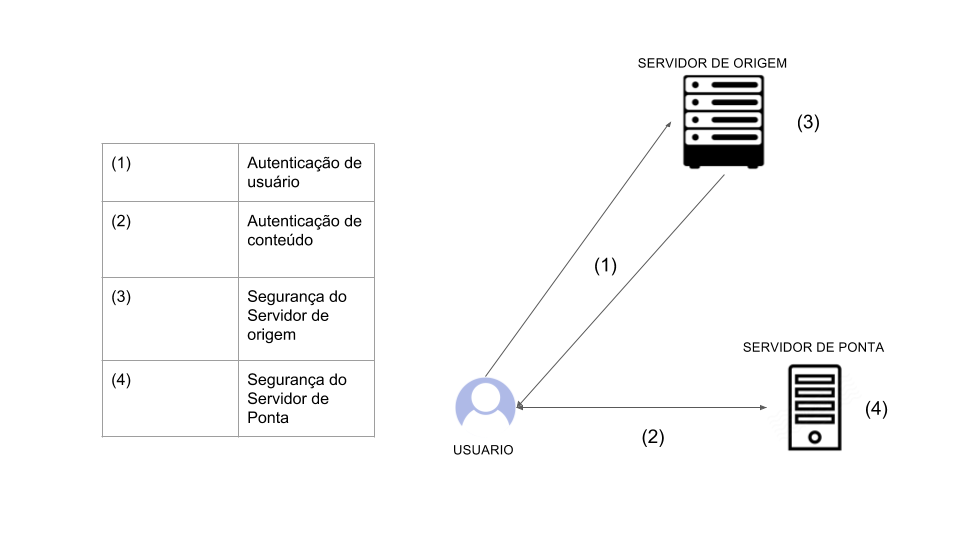
\includegraphics[height=9cm]{Figuras/seguranca_intro.png} 
\label{figura:seguranca_intro}
\end{figure}

Como vemos na figura \ref{figura:seguranca_intro} podemos observar se tem quatro principais pontos a serem garantidos em uma rede. O primeiro trata-se da autentica\c{c}\~ao de usu\'ario que \'e capacidade do sistema de garantir que aquele usu\'ario que est\'a acessando o conte\'udo tem mesmo os requisitos para acess\'a-lo. Ou seja, \'e mesmo um usu\'ario do sistema. Por ser um tema bem abrangente ser\'a tratado com mais profundidade em \ref{subsection:autenticacao_usuario}.
\paragraph{}
Em segundo lugar temos a autentica\c{c}\~ao de conte\'udo. Que \'e a garantia que o conte\'udo acessado \'e o mesmo buscado pelo usu\'ario, que o usu\'ario tem acesso a ele e tamb\'em \'e um conte\'udo que faz parte da rede de disponibilidade da CDN(que n\~ao \'e um conte\'udo inserido por terceiro sem autoriza\c{c}\~ao pr\'evia). Tudo isso tem que ser minuciosamente tratado e averiguado antes de retornar ao usu\'ario. Tudo isso ser\'a abordado em \ref{subsection:autenticacao_conteudo}.
\paragraph{}
Nos dois outros, (3) e (4), trata-se da seguran\c{c}a dos servidores. A\'i podemos falar de seguran\c{c}a f\'isica e l\'ogica. Tem-se que levar em conta a forma de acesso de cada um na hora de mensurar os aspectos de seguran\c{c}a de cada um deles. 
\paragraph{}
No servidor de origem se tem um acesso via DNS, com um endereço "leg\'ivel". Esse acesso se dar\'a muitas vezes por v\'arias parte do globo, tendo que deix\'a-lo dispon\'ivel , portanto, vulner\'avel \`a diversos tipos de ataque, o qu\^e o torna extremamente complexo na hora de definir suas regras de seguran\c{c}a, n\~ao basta apenas subir um \textit{firewall} bloqueando m\'ultiplos acessos, \'e preciso saber exatamente os tipos de aplica\c{c}\~oes que ser\~ao tratadas para assim come\c{c}ar a desenhar as regras de \textit{firewall} que ser\~ao aplicadas, e tamb\'em, na maioria dos casos, ser\'a necess\'ario a implementa\c{c}\~ao de protocolos de prote\c{c}\~ao dentro da pr\'opria aplica\c{c}\~ao que rodar\'a no servidor.
\paragraph{}
J\'a no servidor de ponta a preocupa\c{c}\~ao com o acesso via DNS j\'a \'e uma coisa a menos, visto que muitas vezes o acesso funcionar\'a via redirecionamento do servidor de origem, sendo o controle de endere\c{c}o feito pelo o mesmo. Mas h\'a diversos outros aspectos que tem que serem levados em conta, como parte da autentica\c{c}\~ao de conte\'udo para o usu\'ario, que nada mais \'e que garantir que o usu\'ario para o qual est\'a sendo enviado o conte\'udo tem acesso ao mesmo. Outra grande preocupa\c{c}\~ao \'e quanto a sua disponibilidade, pois \'e necess\'ario que o mesmo esteja "de p\'e" quando for requisitado conte\'udo e que durante o processo de transfer\^encia, caso haja alguma interrup\c{c}\~ao a mesma seja informada ao servidor de origem e o usu\'ario transferido para outro servidor sem que haja muitos danos \`a experi\^encia. Isso sem contar nas enumeras preocupa\c{c}\~oes que se deve ter com servidores. No livro \cite{stallings1995network} se pode aprofundar um pouco mais nessas quest\~oes de seguran\c{c}a na \textit{web}.
\paragraph{}
Mas para se aprofundar um pouco mais dentro dos conceitos de seguran\c{c}a de usu\'ario e conte\'udo de uma CDN \'e necess\'ario primeiro conhecer um pouco sobre protocolos AAA e ter as defini\c{c}\~oes de seguran\c{c}a muito bem esclarecidas, pois assim esses conte\'udos o ser\~ao mais diger\'iveis. Ambos temas ser\~ao tratado em \ref{subsection:AAA} e \ref{subsection:definicoes_seguranca} respectivamente.
\subimport{seguranca/}{AAA}
\subimport{seguranca/}{definicoesseguranca}
\subimport{seguranca/}{autenticacaousuario}
\subimport{seguranca/}{autenticacaoconteudo}

\section{References}

\bibliographystyle{sbc}
\bibliography{sbc-template}

\end{document}
